\chapter{Opis platformy sprzętowej}

\section{Specyfikacja sprzętowa platformy Zybo}

\begin{figure}[h]
	\centering
	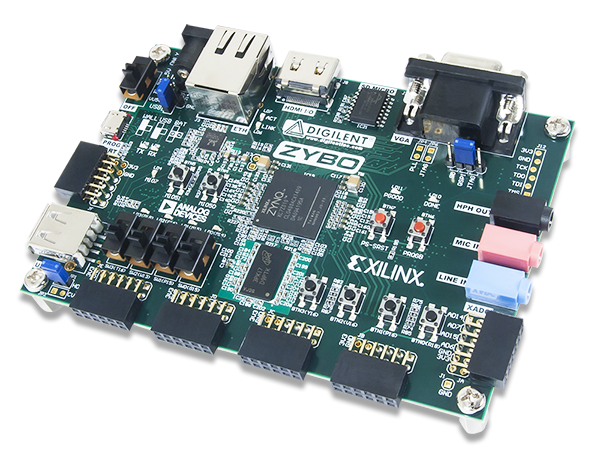
\includegraphics[scale=2]{zybo_img.png}
	\caption{Platforma Zybo z~układem Zynq SoC. Źródło: \cite{zybo_img}}
	\label{fig:zybo_img}
\end{figure}

Do implementacji sprzętowej została wykorzystana karta Zybo firmy Digilent \ref{fig:zybo_img} wyposażona w~układ Zynq SoC (ang. \textit{System on Chip}). 
W~dokumencie \cite{zybo_description} znajduje się opis budowy układu. 
Jest on określany mianem "heterogeniczny", ponieważ zawiera dwa rodzaje zasobów sprzętowych: dwurdzeniowy procesor ARM Cortex-A9 oraz układ FPGA(ang.\textit{Field Programmable Gate Array} -- bezpośrednio programowalna macierz bramek), czyli logikę reprogramowalną.

\subsection{Logika reprogramowalna}



Część reprogramowalna układu Zynq na karcie Zybo jest oparta o~logikę serii  Artix-7 firmy Xilinx. 
Podstawowym elementem z~którego zbudowane jest FPGA, to blok CLB (ang. \textit{Configurable Logic Block}). 
Składa się on z~dwóch Slice'ów połączonych z~matrycą przełączeń (ang. \textit{Switch Matrix}). 
W~układach Zynq występują dwa rodzaje elementów Slice, są to SliceL i SliceM. 
Slice typu M składa się z:
\begin{itemize}
	\item generatora funkcyjnego (4 sztuki) -- został on zrealizowany przy pomocy układów LUT (ang. \textit{Look-Up Table}). Posiada 6 wejść i~2 wyjścia. Może także zostać skonfigurowany jako synchroniczna pamięć RAM lub 32 bitowy rejestr przesuwny wykorzystywany w~liniach opóźniających,
	\item przerzutnika typu D (FF -- ang. \textit{Flip-Flop}) -- slice zawiera 8 sztuk, przy czym 4 mogą zostać skonfigurowane jako zatrzask (ang. \textit{latch}),
	\item multiplekserów,
	\item szybkiej logiki przeniesienia.
\end{itemize}

Do pozostałych zasobów dostępnych w układach FPGA serii Artix-7 należą:
\begin{itemize}
	\item CMT (ang. \textit{Clock Managment Tiles}) -- bloki umożliwiające zarządzanie sygnałem zegarowym, generowanie różnych częstotliwości zegara, równomierną propagację sygnału, tłumienie zjawiska zakłócenia fazy zegara,
	\item Block RAM (BRAM) -- blokowa dwuportowa pamięć RAM o~rozmiarze 36Kb (na blok). Może zostać skonfigurowana jako moduł FIFO (ang. \textit{First In First Out}),
	\item DSP48A1 -- moduł zawierający mnożarkę 25x18 bitów oraz akumulator 48 bitowy. Liczba modułów zależy od rozmiaru układu i~zawiera się w przedziale od 66 do 2020,
	\item Select I/O -- banki zasobów wejścia/wyjścia, których liczba zawiera się w~przedziale od 100 do 400 końcówek podłączonych do części FPGA, 
	\item GTP/GTX Transceivers -- moduły umożliwiające transmisję szeregową z~prędkością do 12,5 Gb/s (GTX) i~6,25 (GTP).
\end{itemize}

\subsection{System procesorowy}
ARM Cortex-A9 MPCore jest 32 bitowym procesorem firmy ARM Holdings z~zaimplementowaną archtekturą ARMv7-A. 
Zawiera od 1 do 4 rdzeni. 
Płytka Zybo Zynq SoC jest wyposażona w~wersje procesora dwurdzeniowego.
Rozkazy procesorów ARM są tak skonstruowane, aby wykonywały jedną określoną operację w~jednym cyklu maszynowym.
Kluczowymi cechami rdzenia Cortex-A9 są \cite{armCortex}:

\begin{itemize}
	\item NEON SIMD (ang. \textit{single instruction, multiple data} -- pojedyncza instrukcja, wiele danych) opcjonalne rozszerzenie zestawu instrukcji do 16 operacji na instrukcję,
	\item jednostka zmiennoprzecinkowa VFPv3 dwukrotnie przewyższająca wydajność swojego poprzednika ARM FPUs,
	\item kodowanie zestawu instrukcji Thumb-2 zmniejsza rozmiar programów, co poprawia wydajność,
	\item rozszerzenia zabezpieczeń TrustZone,
	\item program Trace Macrocell i~CoreSight Design Kit do nieinwazyjnego śledzenia wykonywania instrukcji,
	\item kontroler pamięci podręcznej L2 (0-4 MB),
	\item przetwarzanie wielordzeniowe,
	\item kontroler pamięci statycznej, dynamicznej i bezpośredniej.
\end{itemize}
